\let\negmedspace\undefined
\let\negthickspace\undefined
\documentclass[journal]{IEEEtran}
\usepackage[a5paper, margin=10mm, onecolumn]{geometry}
%\usepackage{lmodern} % Ensure lmodern is loaded for pdflatex
\usepackage{tfrupee} % Include tfrupee package

\setlength{\headheight}{1cm} % Set the height of the header box
\setlength{\headsep}{0mm}     % Set the distance between the header box and the top of the text

\usepackage{gvv-book}
\usepackage{gvv}
\usepackage{cite}
\usepackage{amsmath,amssymb,amsfonts,amsthm}
\usepackage{algorithmic}
\usepackage{graphicx}
\usepackage{textcomp}
\usepackage{xcolor}
\usepackage{txfonts}
\usepackage{listings}
\usepackage{enumitem}
\usepackage{mathtools}
\usepackage{gensymb}
\usepackage{comment}
\usepackage[breaklinks=true]{hyperref}
\usepackage{tkz-euclide} 
\usepackage{listings}
% \usepackage{gvv}                                        
\def\inputGnumericTable{}                                 
\usepackage[latin1]{inputenc}                                
\usepackage{color}                                            
\usepackage{array}                                            
\usepackage{longtable}                                       
\usepackage{calc}                                             
\usepackage{multirow}                                         
\usepackage{hhline}                                           
\usepackage{ifthen}                                           
\usepackage{lscape}
\begin{document}

\bibliographystyle{IEEEtran}
\vspace{3cm}

\title{NCERT - 10.4.ex.18}
\author{EE24BTECH11040 - Mandara Hosur}
% \maketitle
% \newpage
% \bigskip
{\let\newpage\relax\maketitle}

\renewcommand{\thefigure}{\theenumi}
\renewcommand{\thetable}{\theenumi}
\setlength{\intextsep}{10pt} % Space between text and floats


\numberwithin{equation}{enumi}
\numberwithin{figure}{enumi}
\renewcommand{\thetable}{\theenumi}

\textbf{Question:}\\
Find the discriminant of the equation $3x^2 - 2x + \frac{1}{3} = 0$ and hence find the nature of its roots. Find them, if they are real.

\textbf{Theoretical Solution:}\\
Comparing with the standard form of a quadratic:
\begin{align}
    ax^2 + bx + c = 0 
\end{align}
We see that $a = 3$, $b = -2$, and $c = \frac{1}{3}$.
Discriminant $D$ is  calculated as:
\begin{align}
    D = b^2 - 4ac = \brak{-2}^2 - 4\brak{3}\brak{\frac{1}{3}} \\
    \implies D = 0
\end{align}
Since $D = 0$, the given quadratic equation has a single real solution. \\
From the quadratic formula, the solution $x$ can be found as follows:
\begin{align}
    x = \frac{-b \pm \sqrt{D}}{2a} \\
    \implies x = \frac{-b}{2a} \\
    \implies x = \frac{-\brak{-2}}{2\brak{3}} \\
    \implies x = \frac{1}{3} = 0.3333333333333333
\end{align}

\textbf{Newton-Raphson Method:}\\
The formula for this method is:
\begin{align}
    x_{n+1} = x_n - \frac{f\brak{x_n}}{f^\prime\brak{x_n}}
\end{align}
As per the given quadratic equation, define:
\begin{align}
    f\brak{x} = 3x^2 - 2x + \frac{1}{3} \\
    f^\prime\brak{x} = 6x - 2
\end{align}
Therefore, the update equation for the Newton-Raphson method becomes:
\begin{align}
    x_{n+1} = x_n - \frac{3x_n^2 - 2x_n + \frac{1}{3}}{6x_n - 2}
\end{align}
Starting with an arbitrary initial guess $x_0 = 0$, $x$ eventually converges to $0.3333326975492664$ after $100$ iterations. Therefore, by Newton-Raphson method:
\begin{align}
    x = 0.3333326975492664
\end{align}

\textbf{Companion Matrix:}\\
Companion matrix can be written as
\begin{align}
    C = \myvec{0 & \frac{-c}{a} \\ 1 & \frac{-b}{-a}} \\
    \implies C = \myvec{0 & \frac{1}{9} \\ 1 & \frac{2}{3}}
\end{align}
The eigenvalues of $C$ are the roots of the given quadratic equation. The QR algorithm can be used to find the eigenvalues of $C$. \\
The QR algorithm repeatedly factorises the matrix $C$ as:
\begin{align}
    C = Q_kR_k
\end{align}
Here, $Q_k$ is an orthogonal matrix (from QR decomposition) and $R_k$ is an upper triangular matrix. \\
The next iteration is
\begin{align}
    C_{k+1} = R_kQ_k
\end{align}
This process continues until the off-diagonal elements become negligibly small, revealing the eigenvalues of $C$ along the diagonal. \\
Using this method and running $1000$ iterations, the obtained eigenvalues are $0.3336667$ and $0.33299997$, which are both close. Taking their average, 
\begin{align}
    x = \frac{0.3336667+0.33299997}{4} = 0.333333335
\end{align}

\textbf{Fixed-Point Iteration:}\\
The fixed-point iteration method is based on rewriting the equation $f\brak{x}=0$ in the form $x=g\brak{x}$, and iterating (until convergence) using the update equation
\begin{align}
    x_{n+1} = g\brak{x_n}
\end{align}
As per the given quadratic equation, we have:
\begin{align}
    x = \frac{3x^2 + \frac{1}{3}}{2}
\end{align}
Therefore, the update equation is
\begin{align}
    x_{n+1} = \frac{3x_n^2 + \frac{1}{3}}{2}
\end{align}
Iterating 100 times, taking initial guess $x_0 = 0$, we get
\begin{align}
    x = 0.32706948008625647
\end{align}

\newpage

\textbf{Plot:}
\begin{figure}[h]
	\centering
	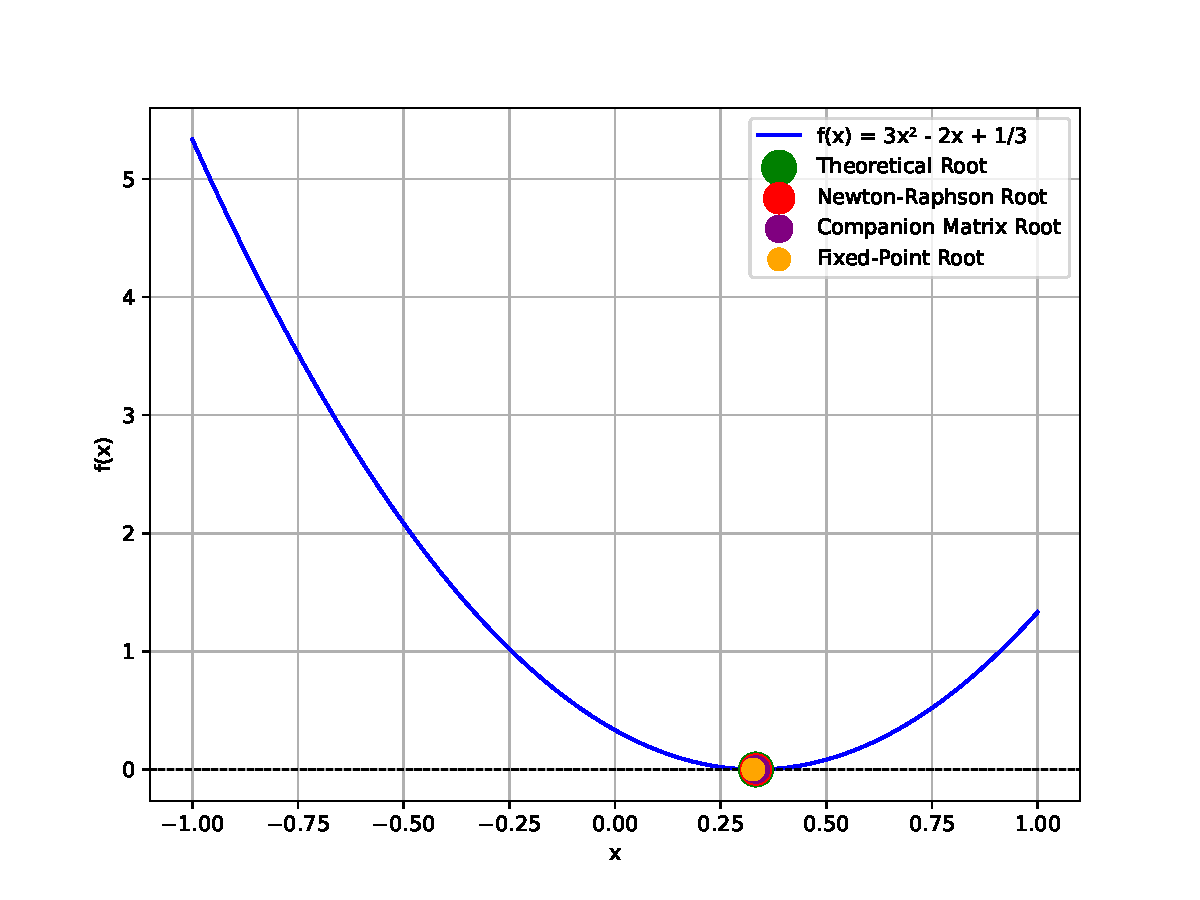
\includegraphics[width=\columnwidth]{figs/fig.pdf}
	\caption{Plot}
\end{figure}

\end{document}
